\documentclass[tikz,border=8pt]{standalone}
\usepackage{amsmath}
\usetikzlibrary{arrows.meta,calc}

\definecolor{axisgray}{RGB}{95,99,104}
\definecolor{positiveblue}{RGB}{66,133,244}
\definecolor{negativeorange}{RGB}{230,126,34}
\definecolor{singularred}{RGB}{192,57,43}

\begin{document}
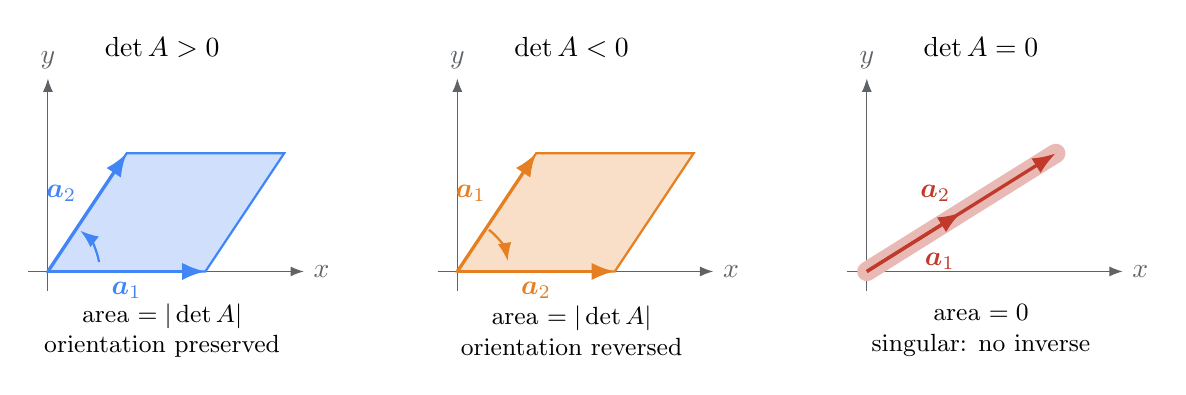
\begin{tikzpicture}[
  >=Latex,
  axis/.style={->, thin, axisgray},
  vector/.style={->, very thick},
  panel title/.style={font=\bfseries},
  note/.style={font=\small, align=center}
]

% Positive determinant: orientation preserved.
\begin{scope}[xshift=0cm]
  \draw[axis] (-0.25,0) -- (3.25,0) node[right] {$x$};
  \draw[axis] (0,-0.25) -- (0,2.45) node[above] {$y$};
  \coordinate (O) at (0,0);
  \coordinate (A) at (2,0);
  \coordinate (B) at (1,1.5);
  \coordinate (C) at (3,1.5);
  \fill[positiveblue!25] (O) -- (A) -- (C) -- (B) -- cycle;
  \draw[positiveblue, thick] (O) -- (A) -- (C) -- (B) -- cycle;
  \draw[vector, positiveblue] (O) -- (A) node[midway, below] {$\boldsymbol a_1$};
  \draw[vector, positiveblue] (O) -- (B) node[midway, above left] {$\boldsymbol a_2$};
  \draw[->, positiveblue, thick] (0.65,0.12) arc[start angle=10,end angle=52,radius=0.65];
  \node[panel title] at (1.45,2.85) {$\det A>0$};
  \node[note] at (1.45,-0.75) {area $=|\det A|$\\orientation preserved};
\end{scope}

% Negative determinant: same area, reversed orientation.
\begin{scope}[xshift=5.2cm]
  \draw[axis] (-0.25,0) -- (3.25,0) node[right] {$x$};
  \draw[axis] (0,-0.25) -- (0,2.45) node[above] {$y$};
  \coordinate (O) at (0,0);
  \coordinate (A) at (1,1.5);
  \coordinate (B) at (2,0);
  \coordinate (C) at (3,1.5);
  \fill[negativeorange!25] (O) -- (A) -- (C) -- (B) -- cycle;
  \draw[negativeorange, thick] (O) -- (A) -- (C) -- (B) -- cycle;
  \draw[vector, negativeorange] (O) -- (A) node[midway, above left] {$\boldsymbol a_1$};
  \draw[vector, negativeorange] (O) -- (B) node[midway, below] {$\boldsymbol a_2$};
  \draw[->, negativeorange, thick] (0.40,0.53) arc[start angle=52,end angle=10,radius=0.65];
  \node[panel title] at (1.45,2.85) {$\det A<0$};
  \node[note] at (1.45,-0.75) {area $=|\det A|$\\orientation reversed};
\end{scope}

% Zero determinant: the parallelogram collapses to a line.
\begin{scope}[xshift=10.4cm]
  \draw[axis] (-0.25,0) -- (3.25,0) node[right] {$x$};
  \draw[axis] (0,-0.25) -- (0,2.45) node[above] {$y$};
  \coordinate (O) at (0,0);
  \coordinate (A) at (1.2,0.75);
  \coordinate (B) at (2.4,1.5);
  \draw[singularred!35, line width=7pt, line cap=round] (O) -- (B);
  \draw[vector, singularred] (O) -- (A) node[midway, below right] {$\boldsymbol a_1$};
  \draw[vector, singularred] (O) -- (B) node[midway, above left] {$\boldsymbol a_2$};
  \node[panel title] at (1.45,2.85) {$\det A=0$};
  \node[note] at (1.45,-0.75) {area $=0$\\singular: no inverse};
\end{scope}

\end{tikzpicture}
\end{document}
